\documentclass{standalone}
\usepackage{tikz}
\usepackage{standalone}
\begin{document}
	
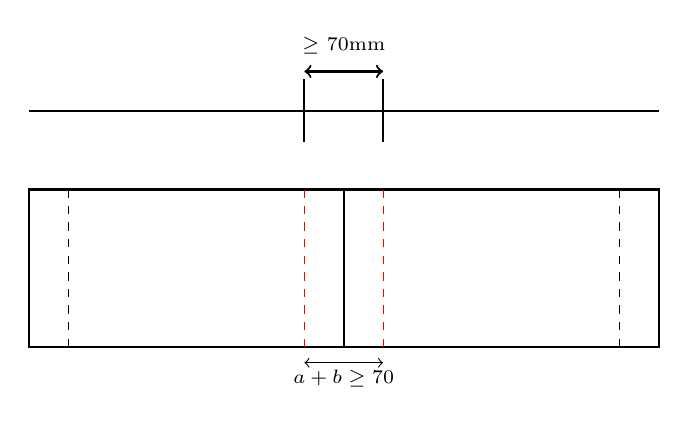
\begin{tikzpicture}
%\draw [help lines] (-1,-2) grid (9,5);

\draw [thick] (0,3) -- (8,3);
\draw [thick] (3.5,3.4) -- (3.5,2.6);
\draw [thick] (4.5,3.4) -- (4.5,2.6);
\draw [thick, <->] (3.5, 3.5) -- (4.5, 3.5);
\node [above] at (4,3.6) {\scriptsize $\geq$ 70mm};


\draw [thick] (0,0) rectangle (8,2);
\draw [thick] (4,2) -- (4,0);
\draw [dashed] (0.5,0) -- (0.5,2);
\draw [red, dashed] (3.5,0) -- (3.5,2);
\draw [red, dashed] (4.5,0) -- (4.5,2);
\draw [dashed] (7.5,0) -- (7.5,2);

\draw [<->] (3.5,-.2) -- (4.5,-.2);
\node at (4, -.4) {\scriptsize $a + b \geq 70$};






\end{tikzpicture}
	
\end{document}